\section{C++ Implementation}
\label{sec:c++_implementation}

Passing from Python to C++ presents some challenges in the design of a suitable architecture for the RL algorithms discussed above. Following the approach of \cite{joshi2008c++}, our main goal has been code reusability, which is based on the important attributes of clarity and elegance of design. In addition, we always kept in mind the possibility the our original design might need to be extended in the future. In some cases we thus favored extendability compared to efficiency. First we describe the C++ adaptation of the PyBrain's \lstinline{Environment}, \lstinline{Task}, \lstinline{Agent} and \lstinline{Experiment} objects with a particular attention to their concrete implementations for the asset allocation problem. Secondly, we discuss the design for an Average-Reward Actor-Critic agent (ARAC), which provides a concrete implementation of the \lstinline{Agent} interface and can be used to solve the asset allocation problem. Here we only give an overview of the program, addressing the reader to the full documentation which can be found at \lstinline{Code/Thesis/doc/doc.pdf} for a thorough explanation of all the classes and their methods. 

\subsection{\lstinline{Environment}, \lstinline{Task}, \lstinline{Agent} and \lstinline{Experiment}}
Figure \ref{fig:class_architecture_base} schematically represents the design of the base components of an RL application, which closely replicates Pybrain's architecture. The pure abstract classes \lstinline{Environment}, \lstinline{Task}, \lstinline{Agent} and \lstinline{Experiment} define the generic interfaces to which all the concrete implementations of these objects must adhere. To achieve code modularity, we make most of the objects in our design clonable in order to allow for the polymorphic composition of classes. Exploiting this design pattern, we couple a \lstinline{Task} with an \lstinline{Environment} by storing a \lstinline{std::unique_ptr<Environment>} as a private member of the class. Similarly, an \lstinline{Experiment} is coupled via composition with a \lstinline{Task} and an \lstinline{Agent}. The methods of these classes are similar to those in Pybrain. For all the linear algebra operations we decided to use Armadillo\footnote{\url{http://arma.sourceforge.net/}}, a high quality linear algebra library which provides high-level syntax (API) deliberately similar to Numpy and Matlab aiming towards a good balance between speed and ease of use. Therefore, the state of the system and the actions performed by the agent are represented as \lstinline{arma::vector} objects.
\begin{sidewaysfigure}[h!]
    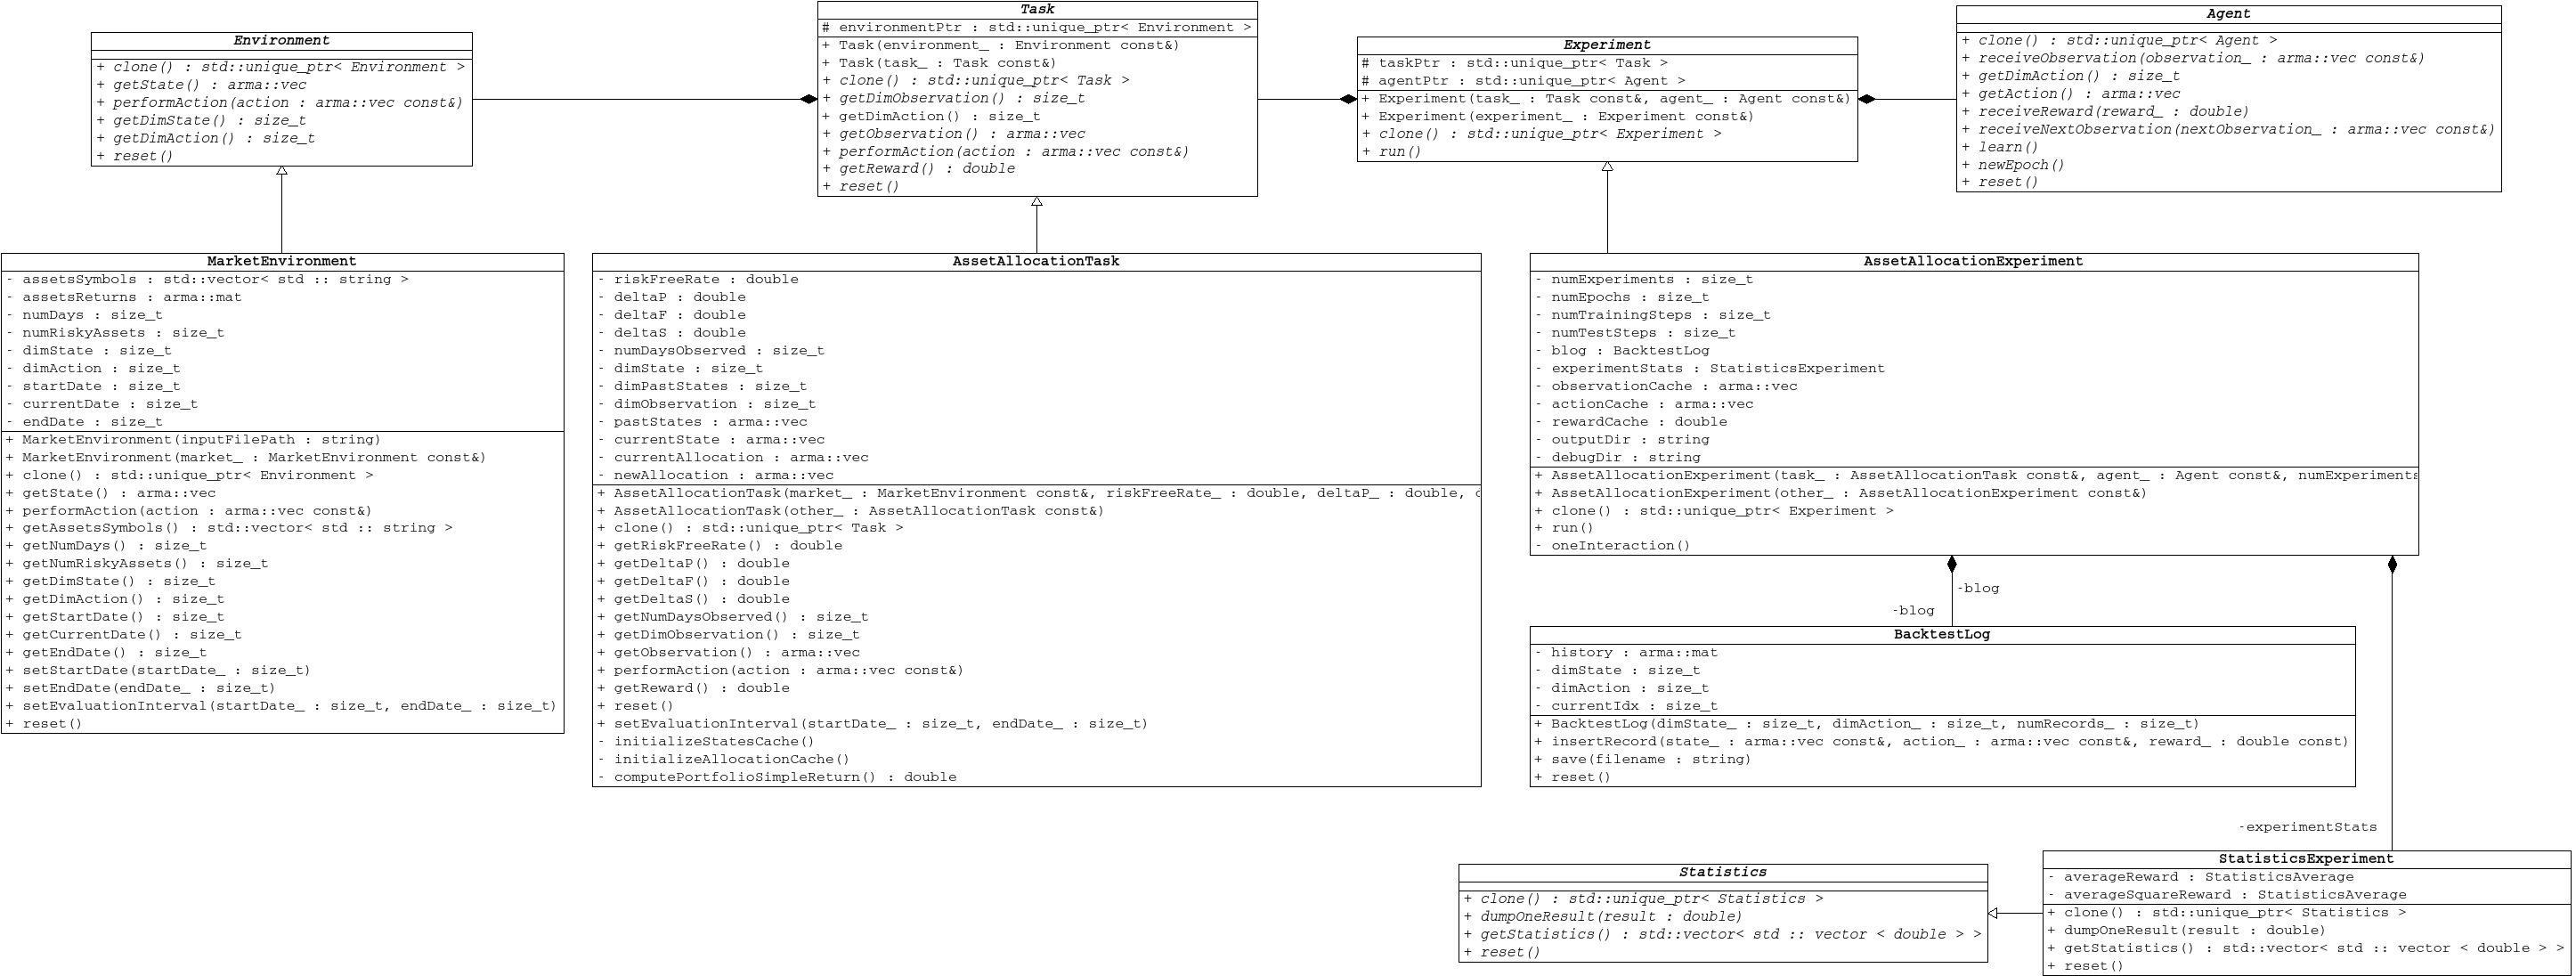
\includegraphics[width=\textwidth]{Images/agent_environment_interaction}
    \caption{Class architecture for the learning process in the asset allocation problem.}
    \label{fig:class_architecture_base}
\end{sidewaysfigure}
Let us now present the concrete implementation of these objects for the asset allocation task. \lstinline{MarketEnvironment} implements a financial market by storing the historical daily returns of the risky assets in an \lstinline{arma::matrix}. These values are read from a given input \lstinline{.csv} file, which is generated automatically running a Python script and which either contains real historical returns downloaded from Yahoo Finance\footnote{\url{https://uk.finance.yahoo.com/}} or synthetic returns generated according to a certain stochastic process. Therefore, we always work on samples of the system without making any assumption on its Markov transition kernel.\clearpage
The \lstinline{AssetAllocationTask} implements the asset allocation MDP discussed in Section \ref{sec:application_to_systematic_trading} by providing a method to compute the reward that the \lstinline{Agent} obtains from investing on the risky assets. Moreover, the \lstinline{AssetAllocationTask} enlarges the system state so that the \lstinline{Agent} also observes the past $P$ states and the current portfolio weights. 
The \lstinline{AssetAllocationExperiment} handles the interactions between the \lstinline{Agent} and the \lstinline{Agent}. The learning process is divided in two phases: the training phase consists of a certain number of learning epochs over the same time period during which the \lstinline{Agent} improves the parameters of its policy via the \lstinline{learn} method. Some estimates of the objective function are dumped in the \lstinline{StatisticsExperiment} object and are used in the post-processing phase to plot the learning curves of the algorithm. In the backtest phase, the \lstinline{Agent} applies the learned policy on the time period which follows the one used for training and the relevant performance measures are stored in the \lstinline{BacktestLog} for successive analysis and comparison between different learning algorithms.

\subsection{\lstinline{ARACAgent}}
A concrete implementation of the \lstinline{Agent} interface completes the standard structure of an RL task. In this section we discuss the design for an Average Reward Actor-Critic agent (ARAC), which includes most of the features of the other algorithms tested in this thesis. The full architecture of this agent is illustrated in Figure \ref{fig:class_architecture_arac}, but for brevity we will only focus on the more interesting aspects.\\
The \lstinline{ARACAgent} builds upon a \lstinline{StochasticActor} and a \lstinline{Critic} via composition. A \lstinline{StochasticActor} is simply a wrapper around a \lstinline{StochasticPolicy}, a pure abstract class defining the generic interface for a stochastic policy used by an agent to select actions. In addition to \lstinline{getAction} and get/set methods for the policy parameters, a \lstinline{StochasticPolicy} must implement the \lstinline{likelihoodScore} method which computes the likelihood score $\nabla_\theta \log \pi_\theta(s,a)$ for a given state and action and which plays a crucial role in any policy gradient algorithm.\\
We provide two examples of concrete implementations of the \lstinline{StochasticPolicy}. The first example is the \lstinline{BoltzmannPolicy} typically used in discrete action spaces. The implementation of this policy is quite straightforward and we won't discuss the details. The second and more interesting stochastic policy implemented is the \lstinline{PGPEPolicy}. This class is based on the decorator design pattern which is typically used to extend the interface of a certain class. Indeed, the \lstinline{PGPEPolicy} is a \lstinline{StochasticPolicy} which contains by polymorphic composition a \lstinline{Policy}, a pure abstract class which provides the generic interface for a policy, potentially deterministic. This \lstinline{Policy} object represents the deterministic controller $F_\theta$ used in the PGPE algorithm. Moreover, the \lstinline{PGPEPolicy} contains by polymorphic composition a \lstinline{ProbabilityDistribution}, a pure abstract class defining the generic interface for a probability distribution. This probability distribution represents the hyper-distribution $p_\xi$ on the controller parameters. In order to be used in a PGPE algorithm, a \lstinline{ProbabilityDistribution} must implement a \lstinline{likelihoodScore} method to compute the likelihood score of the hyper-distribution $\nabla_\xi \log p_\xi(\theta)$. Hence, the \lstinline{likelihoodScore} method of \lstinline{PGPEPolicy} simply broadcasts the call to the \lstinline{likelihoodScore} method of its underlying \lstinline{ProbabilityDistribution}. A concrete implementation of a \lstinline{ProbabilityDistribution} is provided by the \lstinline{GaussianDistribution}, which implements a multi-variate and axis-aligned normal distribution $\calN(\mu, \diag(\sigma))$.\\
The objects discussed so far are sufficient to implement an actor-only learning algorithm, potentially using a baseline to evaluate the rewards. A more advanced variance reduction technique consists in using a \lstinline{Critic}, which approximates the value function and provides an evaluation of a given state. The \lstinline{Critic} class is simply a wrapper around a \lstinline{FunctionApproximator} which provides a generic interface for a parametric function $B_\omega(s)$. The key methods of this class are \lstinline{evaluate}, which evaluates the approximator at a given point, and \lstinline{gradient}, which computes its gradient at a given point.\\
Finally, the \lstinline{ARACAgent} employs some \lstinline{LearningRate} to control the speed of the gradient descent optimization algorithm. A naive approach is to use a \lstinline{ConstantLearningRate}, but this leads to a large-variance in the objective function value attained by the stochastic optimization algorithm. A more sensible choice is to use a \lstinline{DecayingLearningRate} which decreases with the number of learning epochs performed by the agent according to $\alpha_n = \frac{a}{n^b}$. In this way, the learning process progressively ``cools down'' (using a simulated annealing terminology) and stabilizes to a given policy. This concludes our quick overview of the class architecture used for this project. In the thesis, other applications and algorithms were considered and we refer the reader to the full document for a more complete discussion.
\begin{sidewaysfigure}[ht]
    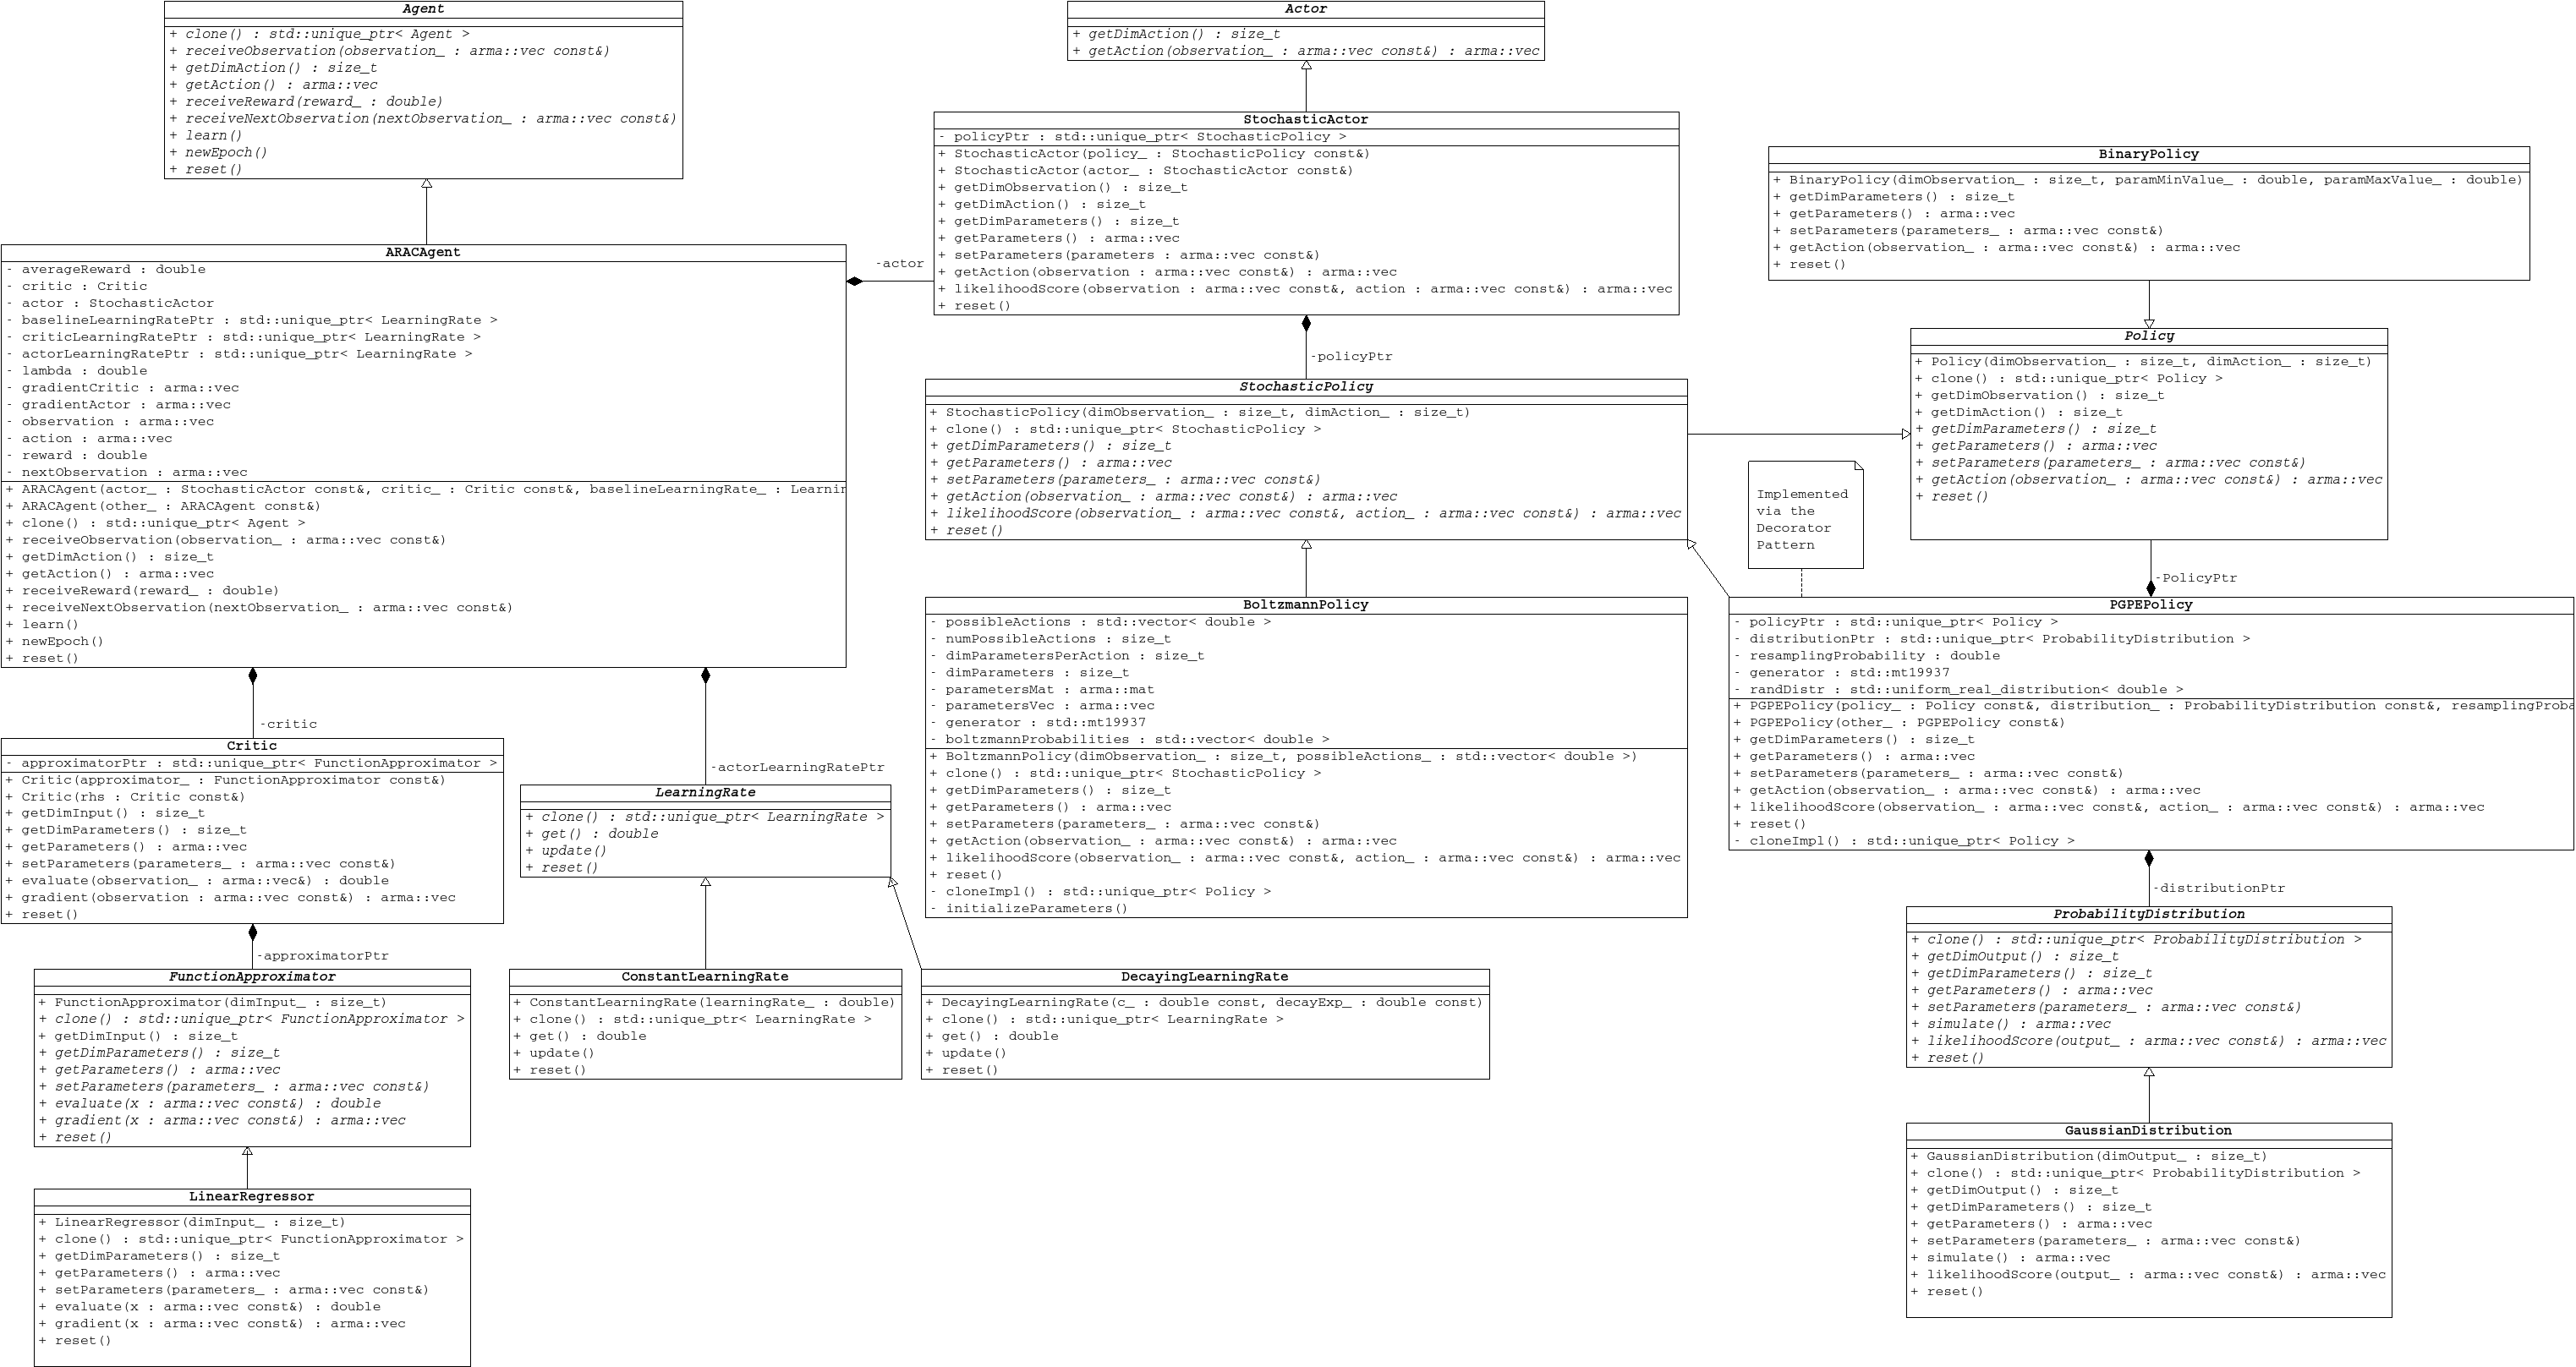
\includegraphics[width=\textwidth]{Images/agent}
    \caption{Class architecture for an Average Reward Actor-Critic agent (ARAC).}
    \label{fig:class_architecture_arac}
\end{sidewaysfigure}

\clearpage